\documentclass[12pt]{puthesis}
%\documentclass[12pt,lot, lof, singlespace]{puthesis}
%\newcommand{\printmode}{}

% Front page materials
\title{Spectroscopic Characterization of New Er$^{3+}$ Host Crystals for Quantum Network Applications}
\submitted{May 2020}  
\copyrightyear{May 2020}  
\author{Henry Allen Ando}
\adviser{Professor Jeff D. Thompson}  
\department{Physics}

% Import packages
\usepackage{graphicx}
\usepackage{verbatim}
\usepackage{multirow}
\usepackage{longtable}
\usepackage{booktabs}
\usepackage{amsmath}
\usepackage{amssymb}
\usepackage{graphicx}
\usepackage{caption}
\usepackage[table,xcdraw]{xcolor}
\usepackage{tikz}
\usepackage{siunitx}
\usepackage{tabularx}
\usepackage{booktabs}
\usepackage[english]{babel}
\usepackage[autostyle, english = american]{csquotes}
\usepackage{siunitx}
\usepackage{float}
\usepackage{array}
\usepackage{paralist}
\usepackage{cite} 
\usepackage{multicol} 
\usepackage{wrapfig}
\usepackage{adjustbox}
\usepackage{physics}
\setlength{\LTcapwidth}{\textwidth}

% Set page geometry options
\usepackage[colorlinks=true,linkcolor=black,citecolor=blue]{hyperref}
\usepackage[margin=1in]{geometry}
\setlength\parindent{28pt}
\usepackage{setspace}
\onehalfspacing

% Define functions
\newcommand{\erbium}[1][ ]{Er$^{3+}$#1}
\newcommand{\YSO}[1][ ]{Y$_{2}$SiO$_{5}$#1}
\newcommand{\ErYSO}[1][ ]{Er$^{3+}$:Y$_{2}$SiO$_{5}$#1}
\newcommand{\TiO}[1][ ]{TiO$_{2}$#1}
\newcommand{\supercite}[1]{$^{\text{\cite{#1}}}$}
\graphicspath{{Figures/}}
\newcommand{\notetoself}[1]{\textcolor{red}{#1}}

% Tweak float placements
\renewcommand{\topfraction}{0.85}  % max fraction of floats at top
\renewcommand{\bottomfraction}{0.6}  % max fraction of floats at bottom
\setcounter{topnumber}{2}
\setcounter{bottomnumber}{2}
\setcounter{totalnumber}{4}  % 2 may work better
\setcounter{dbltopnumber}{2}  % for 2-column pages
\renewcommand{\dbltopfraction}{0.66}  % fit big float above 2-col. text
\renewcommand{\textfraction}{0.15}  % allow minimal text w. figs
\renewcommand{\floatpagefraction}{0.66}	 % require fuller float pages
\renewcommand{\dblfloatpagefraction}{0.66}  % require fuller float pages

% Printed vs. online formatting
\ifdefined\printmode
\usepackage{url}
\else
\ifdefined\proquestmode
\hypersetup{bookmarksnumbered}
\makeatletter
\hypersetup{pdftitle=\@title,pdfauthor=\@author}
\makeatother
\else
\hypersetup{colorlinks,bookmarksnumbered}
\makeatletter
\hypersetup{pdftitle=\@title,pdfauthor=\@author}
\makeatother
\fi % proquest or online formatting
\fi % printed or online formatting

% Enable or disable front matter
\ifodd 1
\renewcommand*{\makecopyrightpage}{}
\renewcommand*{\makeabstract}{}
% \renewcommand{\maketitlepage}{}
\else
\abstract{Large-scale quantum networks will require reliable single-photon sources for distributing entanglement over long distances. The \erbium ion is a good candidate for this purpose as it has an optically accessible transition at 1550 nm, the so-called ``telecom'' wavelength at which light propagates through optical fibers with minimal loss. However, this transition is electric-dipole forbidden and thus spontaneous emission from it is slow (around 100 Hz).
Such a bandwidth constraint would be crippling in a real photonic quantum system. The Thompson lab has bulk-doped \erbium ions into \YSO and then coupled them to silicon nanophotonic cavities, enabling the observation of single photon emissions and enhancing the spontaneous emission rate by a factor of 600 through the Purcell effect \cite{Dibos2017}.
However, the bulk-doped \ErYSO has two downsides. One is that \YSO has strong nuclear spins which limit the  $T_{1}$ and $T_{2}$ spin coherence times of the \erbium ions. The other is that the lower bound on the density of \erbium possible through the bulk-doping process is still too high for individual \erbium ions to be addressed optically.
These issues have motivated a search for new host crystals which can be doped with \erbium through ion implantation, hopefully resulting in substantially lower concentrations of \erbium ions than would be possible through bulk doping. In this work, we characterize the spectral properties of \erbium implanted in various new host crystals, and discuss new techniques for improving the resolution of future such measurements.}
\acknowledgements{Acknowledgements will go here.}
\dedication{To my parents.}
\fi

%%%%%%%%%%%%%%%%%%%%%%%%%%%%%%%%%%%%%%%%%%%%%%%%%%%%%%%%%%%%

\begin{document}
\makefrontmatter

%%%%%%%%%%%%%%%%%%%%%%%%%%%%%%%%%%%%%%%%%%%%%%%%%%%%%%%%%%%%

\chapter{Introduction}
\section{A Brief History of Quantum Computing}

Humans have studied the stars since the beginning of recorded history, and the ancient Greeks were already wondering about the building blocks of reality. Thus, relative to astrophysics or particle physics, quantum computing could be considered a fairly new field. Quantum computers were originally proposed in the early 1980's as a means of simulating quantum many-body problems that are intractible on classical computers \cite{Feynman1982}. The groundwork of the theory was originally laid out largely by Benioff and Feynman \cite{Benioff1980,Feynman1982}. Toffoli created the first set of universal, reversible quantum logic gates \cite{Toffoli1980}. The no-cloning theorem, which states that \textit{qubits}\footnote{ Qubits, short for quantum bits, are two-element quantum spinors. Photon polarization and electron spin are common examples. A quantum computer has several qubits and performs unitary gates on them analogously } cannot be copied, was proved by Wootters and Zurek \cite{Wootters1982}. In 1985, Deutsch proposed the first model for a universal quantum computer \cite{Deutsch1985}.

As the theory developed throughout the 1990's, theorists began to discover problems whose computational complexity could be vastly reduced on quantum computers. The first example, the Deutsch-Josza algorithm for determining whether a black-box function is either constant or balanced, is of little practical use but inspired many later such algorithms \cite{Deutsch1992}. Another important such discovery is Grover's algorithm for database searches, which offers a quadratic speedup over the classical version \cite{Grover1996}. Perhaps the most important of these discoveries, however, was Shor's algorithm (proposed in 1994), which provides an exponential speedup on the discrete logarithm and large integer factorization problems \cite{Shor1994}. Since most modern telecommunications\footnote{ and thus most of the internet.} are encrypted using RSA encryption schemes which rely on the difficulty of factorizing products of large prime numbers, a real quantum computer capable of running Shor's algorithm would instantly break the encryption on almost the entire internet. It was this discovery which catapulted the field of quantum computing from being an interesting physics experiment to a global arms race involving the governments of the United States and China,\footnote{ among others.} as well as tech companies such as Google, IBM, and Microsoft. 

But while quantum computers threaten to break classical factorization-based encryption methods, they create in exchange the possibility for physically un-interceptible encrypted communication. The oldest and most famous of these so-called \emph{quantum cryptography} schemes is the BB84 protocol for quantum key distribution. This protocol, which encodes information in the polarization states of photons, enables one party to send a private key to another in such a way that any attempt to intercept the message would be detectable to the receiver \cite{Bennett2014,Shor2000}. Another uniquely quantum communication procedure is \emph{teleportation}. In quantum teleportation, a qubit is transmitted from one party to another instantaneously across arbitrarily large distances. This doesn't violate the lightspeed limit for the transfer of information, because a qubit isn't information, and because the protocol requires a classical bit to be exchanged beforehand anyway \cite{Bennett1993}. 

\notetoself{Here is a potential spot to talk about error correction. However, I'm not sure it's worth the space/time. For the moment, I'll leave only this reminder.}

Thus far, the theory of quantum algorithms and protocols has ranged far ahead of our ability to physically implement them. Over the years, a few broad classes of physical quantum computers have emerged as the most promising, each for slightly different types of problems. A few of these classes are:
\newcommand{\listheader}[1]{\textbf{#1}}
\begin{itemize}
  
\item \listheader{Trapped ion quantum computers} use the electronic spins of ions trapped in an optical lattice as the qubit \cite{Cirac1995}. Alternatively, trapped neutral atoms can be used, with nuclear spins as the qubits \notetoself{[?]}. The dipole-dipole interactions between adjacent particles can be tuned to perform two-qubit gates, thus making atom trap quantum computers a viable platform for a universal quantum computer \notetoself{[?]}.
  
\item \listheader{Nuclear magnetic resonance (NMR) quantum computers} use the nuclear spins of atoms or molecules dissolved in solution as the qubit \cite{Cory1997}. Unfortunately, it was shown after a few seemingly successful bulk NMR demonstrations that no entanglement had actually occurred in these experiments, and that entangelement is a necessary part of most important quantum algorithms \cite{Braunstein1999,Linden2001}. It was also hard to scale these computers, as each extra qubit required the synthesis of a new molecule. However, the legacy of NMR computers lives on, as many current quantum computing schemes (see the next list item) make use of the main ideas of NMR computers.
  
\item \listheader{Point defects in solid state hosts} such as rare earth ions or nitrogen-vacancy (NV) centers in crystals are in some sense descendents of NMR-based quantum computing paradigms \notetoself{[?]}. In these systems, the spin states of valence electrons serve as qubits. Light-matter interfaces can be achieved by coupling these atoms with photons at the same energy as an optical transition in the qubit atom \notetoself{[?]}. 

\item \listheader{Linear optical quantum computers} use the polarization states of photons as qubits \cite{Knill2001}. The main advantage of this paradigm is that it enables easy transfer of qubits over long distance, because the computational qubits can be sent directly over long distances, either through fiber optic cables or through free space telescopes, with no extra conversion step. 
    
\item \listheader{Superconducting circuit quantum computers} use the phase differences across superconducting Josephson junctions as qubits \cite{Nakamura1999}. These types of computers have so far been the largest, with Google claiming to demonstrate \emph{quantum supremacy} (the ability of a quantum computer to solve a problem faster than a classical counterpart) for the first time on a 53-qubit superconducting quantum computer in 2019 \cite{Arute2019}.
  
\end{itemize}

Although superconducting circuit quantum computers have been the most successful so far in terms of implementing complicated quantum algorithms, they are not so useful for quantum networks applications. Linear optical quantum computers are the best suited for working purely with photonic qubits in quantum networks, but without the superior computing power offered by superconducting circuits can only implement fairly simple tasks. Thus, point defects in solid state hosts are a very exciting platform, as they offer the possibility of light-matter interfaces that could marry the power of superconducting circuit computers with the distance allowed by photons. This would enable a variety of exciting quantum technologies, such as quantum cryptography, quantum-enhanced metrology, and modular quantum computing \cite{Monroe2014}.

\section{\erbium in crystals as a technology for quantum networks }

Single atoms and atom-like defects in crystals have successfully demonstrated a variety of quantum-network-related tasks. Examples include spin-photon entanglement in quantum dots \cite{Greve2012}, entanglement between trapped atoms and photons \cite{Blinov2004}, teleportation between remote trapped atom memories \cite{Nolleke2013}, and spin-photon entanglement using vacancy centers in diamonds \cite{Togan2010}. However, most existing systems use photons in the visible or near-infrared spectrum. For long-distance quantum communications over optical fibers, such photons would suffer crippling losses (on the order of several dB/km). One approach to countering these losses it to use a satellite uplink instead of optical fibers \cite{Yin2017}. However, for a majority of applications a satellite is impractical, and substantial fiber optic infrastructure already exists across the country. Single \erbium ions are thus a very promising qubit for quantum network applications, as they naturally have an optical transition at 1550 nm, the so-called ``telecom'' wavelength where losses in fibers drop to 0.2 dB/km.

This transition, however, is very slow, with a natural linewidth on the order of 100 Hz. For many quantum networking applications, this would be crippling. The relevant times bins for creating indistinguishable photons are on the order of femtoseconds. Even less stringent standards, like the coherence times of many types of qubits, are less than milliseconds. For \erbium based technologies to be viable, their repetition rates need to be increased. 


\begin{figure}[b]
  \centering
  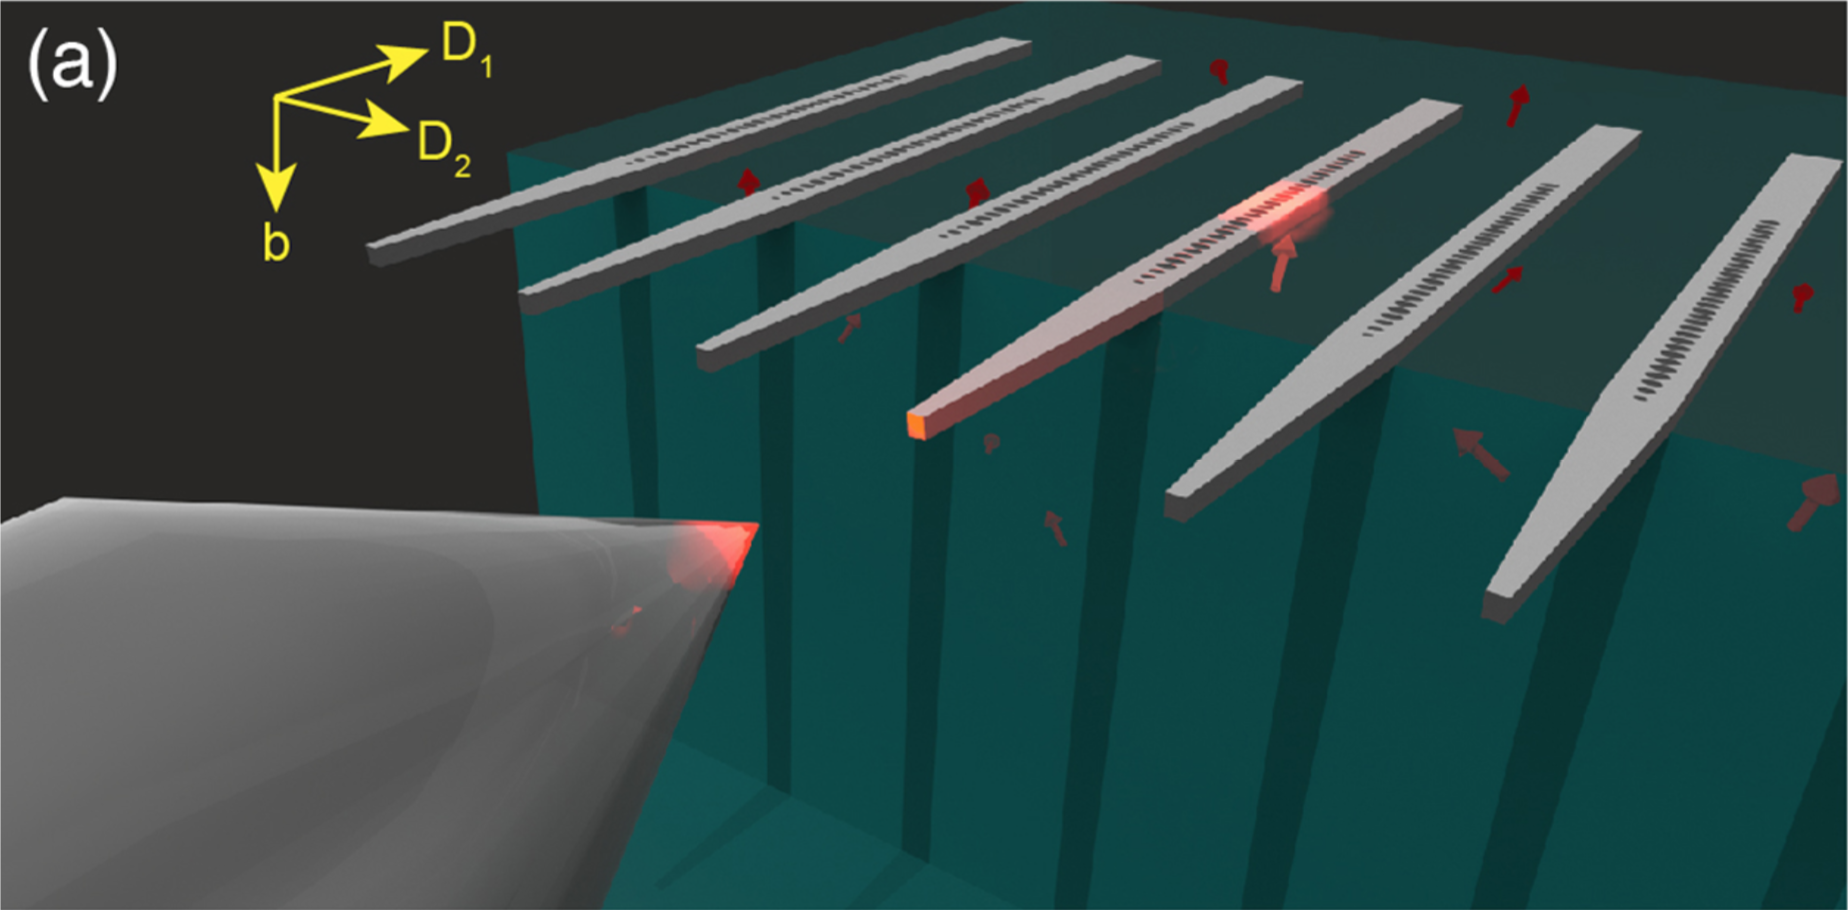
\includegraphics[width=0.8\textwidth]{Nanophotonics}
  \caption{A lensed fiber couples into a silicon photonic cavity stamped on top of an \erbium[]-doped \YSO crystal. Red arrows represent the spins of \erbium ions in the crystal substrate. Figure from \cite{Dibos2017}.}
  \label{fig:cavity}
\end{figure}


Previous work by the Thompson lab has shown that by stamping silicon nanophotonic cavities on top of crystals doped with \erbium ions, the emission rate can be enhanced by 600 times via the Purcell effect \cite{Dibos2017}. Figure \ref{fig:cavity} shows a graphic of this scheme. This approach is very promising - however, the crystal substrate could be improved in numerous ways. For one thing, this work used \YSO[], a crystal with relatively strong nuclear spins. These nuclear spins substantially limit the coherence times of the \erbium spin qubits embedded in the crystal. Another other issue is that the density of \erbium ions is high enough in the bulk-doped \YSO that tens to hundreds of ions couple to the cavity, preventing simple frequency-based resolution of the different ions each cavity couples to, and reducing coherence times further due to electric dipole interactions between nearby \erbium ions. Finally, a different crystal field configuration could potentially increase the emission rate further, by increasing the matrix element between the ground and excited state wavefunctions.\footnote{The \erbium telecom transition is electric dipole forbidden. Small perturbations to the electronic wavefunctions can thus make substantial relative differences to the matrix element between the ground and excited states. The spectroscopic properties of \erbium are discussed in more detail in Section \ref{sec:spectr-prop-erbi}.}

Unfortunately, using bulk doping methods it is impossible to grow crystals with lower concentrations of \erbium than in this previous work \cite{Dibos2017}. The Thompson lab has thus turned to ion implantation to achieve lower doses of \erbium in new potential crystal hosts.\footnote{Ion implantation is a process by which ions are accelerated into the surface of a crystal, and become lodged in the structure of the crystal. More information on this process is given in Section } Last fall, it was shown that \erbium could be successfully implanted in \TiO[], a crystal with low nuclear spins, with narrow optical linewidths \cite{Phenicie2019}. \notetoself{Given that \TiO worked, why continue searching? Not super clear on this myself. Does it have to do with attaching photonic crystals?}

In the interests of discovering potentially more optimal host crystals, a large batch of crystals was implanted with \erbium ions. For all these implanted crystals, it was necessary to determine experimentally whether \erbium was visible in the crystal, and if so, to determine its spectral properties to begin understanding how \erbium ions in this crystal would perform as single photon emitters. Where are the emission and excitation lines? How bright and broad are they? What can we learn about how the \erbium ions are sitting in the crystal lattice? These are the questions that motivate this work.

\section{Spectroscopic Properties of \erbium in Solid State Hosts}
\label{sec:spectr-prop-erbi}

Due to its telecom optical transition, \erbium has a long history of use as a dopant to make telecom wavelength fiber amplifiers.\footnote{Our spectroscopy experiment, in fact, uses an erbium-doped fiber amplifier (EDFA).} This optical transition is between the $^{4}I_{15/2}$ ground state, and an excited state $^{4}I_{13/2}$. This notation, known as spectroscopic notation, takes the form $^{2S+1}L_{J}$, where $S$ is the total spin momentum, $L$ is the total orbital momentum (specified as a letter, $S, P, D,$ etc., where $I$ corresponds to a total orbital momentum of 6), and $J$ is the total angular momentum. 

\begin{wrapfigure}{r}{0.5\textwidth}
  \centering
  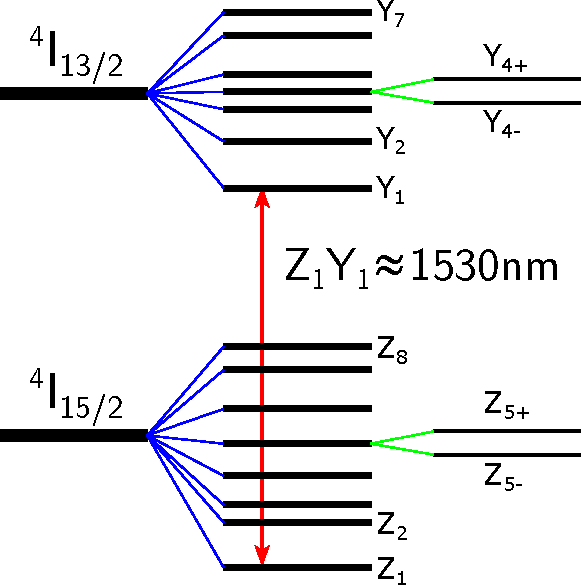
\includegraphics[width=0.48\textwidth]{EnergyLevelDiagram}
  \caption{Diagram showing the Stark splitting due to electric fields within the crystal (blue) and the Zeeman splitting in an applied magnetic field (green). The transition between the lowest ground and excited state levels, labelled in red, typically falls around 1530 nm.}
  \label{fig:energyleveldiagram}
\end{wrapfigure}

There are two consequences to this. One is that, because these $4f$ states lie closer to the nucleus than the $5d$ states which populate earlier, they are relatively shielded from phonons in the crystal. This makes \erbium and other rare-earth ions with this property desirable for building quantum memories, as the coherence times of the optical electrons are unusually good. The second consequence is that this transition is electric-dipole forbidden, as the total angular momentum $L$ is the same in the ground and excited states. This means that the transition is quite slow, with excited state lifetimes on the order of ten milliseconds (as previously discussed). For quantum network applications, this is less than desirable, and one of the principal motivations for the use of silicon photonic cavities. 

Both the ground state and the excited state are degenerate, 16- and 14-fold respectively. In solid state hosts, the crystal fields split these degeneracies via the Stark effect into $J+1/2$ Kramer's doublets. We label the ground state Stark-shifted doublet states with $Z_{1}$ to $Z_{8}$, and the excited state doublets with $Y_{1}$ to $Y_{7}$. In the presence of an applied magnetic field, these doublets themselves are split by the Zeeman effect, and the energy levels can become entirely nondegenerate. This splitting is shown in Figure \ref{fig:energyleveldiagram}. In this work, we ignore the Zeeman splitting, and focus on identifying how the electric field inside the crystal environment shifts the energy levels. 

Because the excited state lifetime of this system is so long, the natural linewidth is quite small. As a result, at low temperatures, the primary line broadening is inhomogeneous, a consequence of slight variations in the locations of different \erbium ions in the crystal, or slight deformations of the crystal field around them.


\section{Crystal fields}

The problem of modeling the effects of crystal fields on the spectra of ions is an old one, and tools exist for approaching it. First, we make use of the central field approximation, which roughly states that the repulsive potential an electron feels due to the other electrons is spherically symmetric. Thus the radial component of the wavefunctions decouples from the angular component, and focus can be turned to the angular component. The key idea underlying crystal field modelling is then decomposing the electric field of the crystal into a sum of spherical harmonics centered on the atom whose perturbations you are trying to measure. In other words, the crystal field hamiltonian is expressed as 
\begin{equation}\label{eq:3}
  H_{CF} = \sum_{k, q}B_{q}^{k}C_{q}^{(k)},
\end{equation}
where $B_{q}^{k}$ are parameters to describe how much of each spherical harmonic is present, and $\mathbf{C}^{(k)}$ are the tensor operators of spherical harmonics \cite{Liu2006}.

The next step is to pick a basis of quantum numbers for describing the angular component of the wavefunctions. The true good quantum numbers in general depend on the relative strength of the electrostatic forces in the atom versus the spin-orbit coupling. However, since the crystal field perturbation will take the form of spherical harmonics, it makes sense to use a basis of simple spherical harmonic wavefunctions. Thus, we use the basis $\ket{l\tau SLJM}$, where $l$ has to do with the radial part of the wavefunction $nl$, $S$ is the total spin momentum, $L$ is the total orbital momentum, $J$ is the total angular momentum $S+L$, and $M$ is the ``magnetic quantum number'' ranging from $-J,-J+1,...,J$, and $\tau$ is a seniority number to distinguish states with the same $S$ and $L$ which can't be otherwise distinguished \cite{Liu2006}.

Having decided on a basis, we do perturbation theory with the crystal field Hamiltonian. This involves computing the matrix elements, which are given by
\begin{equation}\label{eq:4}
  \bra{l\tau SLJM} H_{CF} \ket{l\tau' S'L'J'M'} = \sum_{k, q} B_{q}^{k}(-1)^{J-M}\Bigg(\begin{array}{c c c}J & k & J' \\ -M & q & M'\end{array}\Bigg)D_{J}^{k},
\end{equation}
where
\begin{align}
  D_{J}^{k} =
  & (-1)^{S+L'+J+k}[(2J+1)(2J'+1)]^{1/2}
    \Bigg\{\begin{array}{c c c} J & J' & k \\ L' & L & S \end{array}\Bigg\} \nonumber \\
  & \times \bra{l\tau S L } \mathbf{U}^{(k)}\ket{l\tau' S' L'}(-1)^{l}(2l + 1)
    \Bigg(\begin{array}{c c c} l & k & l \\ 0 & 0 & 0\end{array}\Bigg) \label{eq:5}                                                               
\end{align}
In the above equations, the $()$ and $\{\}$ quantities are 3- and 6-$j$ symbols, a notatation for representing Clebsh-Gordan coefficients. The $\mathbf{U}^{(k)}$ operator is the reduced matrix element of a unit tensor (see \cite{Wybourne1965} for more information). The key conclusion is that these matrix elements can be evaluated exactly and reduced to known linear combinations of the crystal field parameters $B_{q}^{k}$. Calculating the spectrum for a given set of crystal field is then only a matter of diagonalizing the matrix of the crystal field Hamiltonian. As a consequence, if the number of known energy levels is more than the number of unknown crystal field parameters, the crystal field parameters can be found conclusively.

In general, the number of crystal field parameters is infinite. However, various symmetries of the crystal can eliminate many of the possible parameters. For example, if the rare earth ion sees a crystal environment with cubic symmetry, only four crystal field parameters can be nonzero, $B_{4}^{0}$, $B_{4}^{4}$, $B_{6}^{0}$, and $B_{6}^{4}$, and only two of these are actually independent. Thus the problem is a two-parameter one. Lea, Leask and Wolf show an efficient way of calculating the crystal field matrix for diagonalization, 
\begin{equation}\label{eq:7}
  H = B_{4}(O_{4}^{0}+ 5\cdot O_{4}^{4}) + B_{6}(O_{6}^{0}-21\cdot O_{6}^{4}),
\end{equation}
where $O_{4}^{0}$, $O_{4}^{4}$, $O_{6}^{0}$ and $O_{6}^{4}$ are $2J+1$ dimensional constant matrices (for their exact form see \cite{Lea1962}). The upshot of this for our purposes is that the crystal field environment that \erbium ions experience in MgO, a crystal with cubic symmetry, could potentially be determined precisely. In Section \ref{sec:mgo} we take up this task.


%%%%%%%%%%%%%%%%%%%%%%%%%%%%%%%%%%%%%%%%%%%%%%%%%%%%%%%%%%%%


\chapter{Methods}

\section{Sample preparation}
\label{sec:sample-preparation}

\subsection{Ion implantation}
\label{sec:ion-implantation}

\subsection{Annealing}
\label{sec:annealing}


\subsection{Polishing and photonic crystals}
\label{sec:polishing}

\section{Photoluminescence excitation spectroscopy}
\label{sec:phot-excit-spectr}

Photoluminescence excitation spectroscopy (PLE) is a spectroscopy technique wherein the sample is exposed to a tunable excitation laser, and the fluorescence from the sample is collected and measured. In principle, it measures the same physical properties as absorption spectroscopy. However, it is more effective for detecting extremely small doses of a material (as we are dealing with here) because rather than measuring a small signal against a large background, it measures a small signal against almost no background.

PLE spectroscopy measures how much light the sample can absorb and reemit at each wavelength in a scan. Physically, this corresponds to measuring the difference between the energies between the occupied ground states and the energies of the excited states. In theory, there will be excitation peaks at every energy $E_{nm}$ for which there is a transition 
\begin{equation}\label{eq:6}
E_{nm} = Y_{m}-Z_{n}.
\end{equation}
However, the relative strengths of these peaks are modulated by several factors. At different temperatures, the ground states will have different occpancies according to the Boltzmann distribution. The matrix elements between different $Z$ and $Y$ level states can be greater or lesser, which will influence the brightness of the observed transition. Finally, the linewidths of the transitions affect their brightnesses. When the natural linewidth is much smaller than the inhomogeneous linewidth due to environmental factors, only a small fraction of the ions are addressed by the laser at a given moment. On the other hand, as the natural linewidth increases, the excitation efficiency falls, and the line can also become weaker. The balance of these forces can be be unpredictable. Moreover, the laser power is not consistent across all wavelengths due to wavelength-dependent changes in the polarization. Thus, it is currently difficult to draw precise quantitative conclusions based on the relative heights of different excitation peaks. 

\begin{figure}[t]
  \centering
  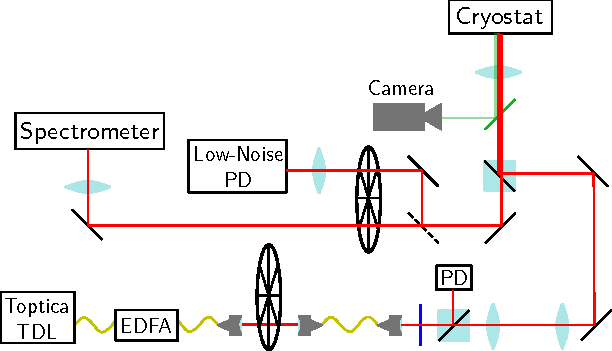
\includegraphics[width=0.9\textwidth]{PLESetupDiagram.pdf}
  \caption{Schematic of our spectroscopy experiment. A half-wave plate is marked in blue, and a dichroic mirror is marked in green. }
  \label{fig:ple}
\end{figure}

Our PLE setup is shown in Figure \ref{fig:ple}. A tunable diode laser is amplified by an erbium-doped fiber amplifier up to \notetoself{200 mW?}. The laser is then passed through a chopper. A half-wave plate (blue) at the output of the fiber enables coarse control over the polarization of the laser before it passes through a polarizing beamsplitter. A photodiode measures the light rejected by the PBS, informing the rotation of the HWP. The laser then passes through a beam expander consisting of two lenses, before reflecting off a PBS towards the vapor cryostat containing the sample. Before the cryostat the laser passes through a lens which focuses it onto the sample surface. A camera, which is added to the beam path with a dichroic (green), helps aim the laser at the sample.

The reflected excitation laser is mostly rejected from continuing down the measurement beampath by virtue of the PBS. Fluorescence from the sample, which has random polarization, makes it through this PBS with 50\% attenuation. The measurement beampath is then directed either to a low-noise photodiode, or to the array detector spectrometer, by inserting or removing a mirror (dotted line). Before measurement, the light passes through a second chopper set to be exactly out of phase with the first, so that residual excitation light is further rejected.\footnote{Since the excitated state lifetime of the \erbium ions is on the order of ms, fluorescent emission continues to be visible for several ms after the excitation laser is blocked.}

When the light is directed into the low-noise photodiode, we are performing pure PLE spectroscopy. There are two modes in which this can be operated. By directing the PD signal to a lock-in amplifier tuned to the frequency of the chopper, we can achieve an extremely low signal-to-noise ratio. This enables the measurement of the smallest signals we can observe with this setup. Alternatively, the PD output can be measured directly, enabling direct observation of the decay of the fluorescence, and thus the excited state lifetime.

In the next section, we discuss the array detector spectrometer and the measurements performed when the signal is instead directed into the other beam path.

\section{Emission spectroscopy with an array detector}
\label{sec:emiss-spectr-with}

\begin{itemize}
\item Why measure emission spectra? Why take 2D spectra? What can you learn from these measurements that you couldn't from just excitation spectroscopy?

\item How does the spectrometer work? 

\item What limits our ability to measure smaller signals with the commercial spectrometer? Why do we think Fourier transform spectroscopy could improve our ability to detect smaller signals?

\item There are other advantages as well - increased range, potentially increased resolution (with larger mirror travel), no need to focus through slit. Putting FT on the excitation side with a broad spectrum source could actually give a way to do 2D spectra over extremely wide regions.
\end{itemize}


\section{Peak finding and assignment}


%%%%%%%%%%%%%%%%%%%%%%%%%%%%%%%%%%%%%%%%%%%%%%%%%%%%%%%%%%%%

\chapter{Characterization of new hosts}


\subsection{MgO}
\label{sec:mgo}

Roughly one to two pages for each material, including:

\begin{itemize}
\item 2D spectrum

\item Table of peak locations

\item Table of proposed energy levels

\item Picture of crystal structure

\item Crystal field parameters (if applicable - probably only MgO)

\item Any additional commentary (unusual lineshapes, etc.)

\item Discussion of potential usefulness for single photon applications 
\end{itemize}


%%%%%%%%%%%%%%%%%%%%%%%%%%%%%%%%%%%%%%%%%%%%%%%%%%%%%%%%%%%%

\chapter{Design of a low-cost, high-resolution Fourier transform spectrometer}

\section{Motivation}



\section{Design}

\subsection{Principles of Fourier transform spectroscopy}
\begin{itemize}
\item A small diagram of how FT spectroscopy works at the simplest level, and a discussion of how data is collected and processed

\item What determines resolution? Range?

\item How does noise work propagate through the Fourier Transform?

\item What is the minimum sampling rate? How do we determine this rate? Nyquist Theorem and DFT 

\item Why use Hann window in Fourier Tranform?
\end{itemize}

\subsection{Implementation}
\begin{itemize}
\item Optical design of our FT spectrometer 

\item Alignment precision and contrast

\item Data collection electronics 

\item Data processing 
\end{itemize}

\subsection{Characterization}
\begin{itemize}
\item Resolution

\item Signal to noise 

\item Future characterization, which was blocked due to coronavirus 

\item Will this be a useful part of the experiment?
\end{itemize}


%%%%%%%%%%%%%%%%%%%%%%%%%%%%%%%%%%%%%%%%%%%%%%%%%%%%%%%%%%%%

\chapter{Conclusions}




%%%%%%%%%%%%%%%%%%%%%%%%%%%%%%%%%%%%%%%%%%%%%%%%%%%%%%%%%%%%

\singlespacing
\bibliographystyle{prsty}
\cleardoublepage
\ifdefined\phantomsection
  \phantomsection  % makes hyperref recognize this section properly for pdf link
\else
\fi
\addcontentsline{toc}{chapter}{Bibliography}
\bibliography{thesis}

\end{document}
